\chapter{Technical Background}
\label{sec:state}

% Hier werden zwei wesentliche Aufgaben erledigt:

% 1. Der Leser muß alles beigebracht bekommen, was er zum Verständnis
% der späteren Kapitel braucht. Insbesondere sind in unserem Fach die
% Systemvoraussetzungen zu klären, die man später benutzt. Zulässig ist
% auch, daß man hier auf Tutorials oder Ähnliches verweist, die hier auf
% dem Netz zugänglich sind.

% 2. Es muß klar werden, was anderswo zu diesem Problem gearbeitet
% wird. Insbesondere sollen natürlich die Lücken der anderen klar
% werden. Warum ist die eigene Arbeit, der eigene Ansatz wichtig, um
% hier den Stand der Technik weiterzubringen? Dieses Kapitel wird von
% vielen Lesern übergangen (nicht aber vom Gutachter ;-), auch später
% bei Veröffentlichungen ist "Related Work" eine wichtige Sache.

% Viele Leser stellen dann später fest, daß sie einige der Grundlagen
% doch brauchen und blättern zurück. Deshalb ist es gut,
% Rückwärtsverweise in späteren Kapiteln zu haben, und zwar so, daß man
% die Abschnitte, auf die verwiesen wird, auch für sich lesen
% kann. Diese Kapitel kann relativ lang werden, je größer der Kontext
% der Arbeit, desto länger. Es lohnt sich auch! Den Text kann man unter
% Umständen wiederverwenden, indem man ihn als "Tutorial" zu einem
% Gebiet auch dem Netz zugänglich macht.

% Dadurch gewinnt man manchmal wertvolle Hinweise von Kollegen. Dieses
% Kapitel wird in der Regel zuerst geschrieben und ist das Einfachste
% (oder das Schwerste weil erste).

%\ldots state of the art \ldots

%\todo{write state}
This chapter offers background knowledge for all the content and topics covered in the thesis. The reader is assumed to understand operating systems, Kubernetes\cite*{k8s}, and confidential computing. Nonetheless, it provides a concise overview of essential terms and concepts to facilitate the reader's 
comprehension of subsequent chapters.

\section{Kubernetes and runtime communication interface}
\label{sec:k8s}
Kubernetes~\cite*{k8s} is a portable and scalable open-source platform for managing and orchestrating containerized workloads. It comprises at least one master node and multiple worker nodes. The master node assumes global decision-making, scheduling, detection, and managing cluster events. As shown in Figure~\ref{fig:k8s}, 
the master node hosts an API server that provides users with an interface to manage and control the cluster. Users can submit requests to update or create Kubernetes objects like pods. A pod represents the smallest deployment unit in Kubernetes, which may encompass multiple containers sharing network 
and storage resources. Moreover, each worker node runs a Kubelet, a daemon responsible for processing requests from the master node and executing services on the node. When handling container creation and image management requests, Kubelet invokes a high-level container runtime like 
Containerd~\cite*{containerd} or CRI-O~\cite*{cri-o}.These high-level runtimes take charge of managing the container lifecycle and images while delegating pod creation and 
deletion to lower-level OCI-compliant runtimes such as Kata~\cite*{Kata-Containers}, Quark~\cite*{quark}, RunC~\cite*{runc}, etc.
\begin{figure}[htp]
  \centering
  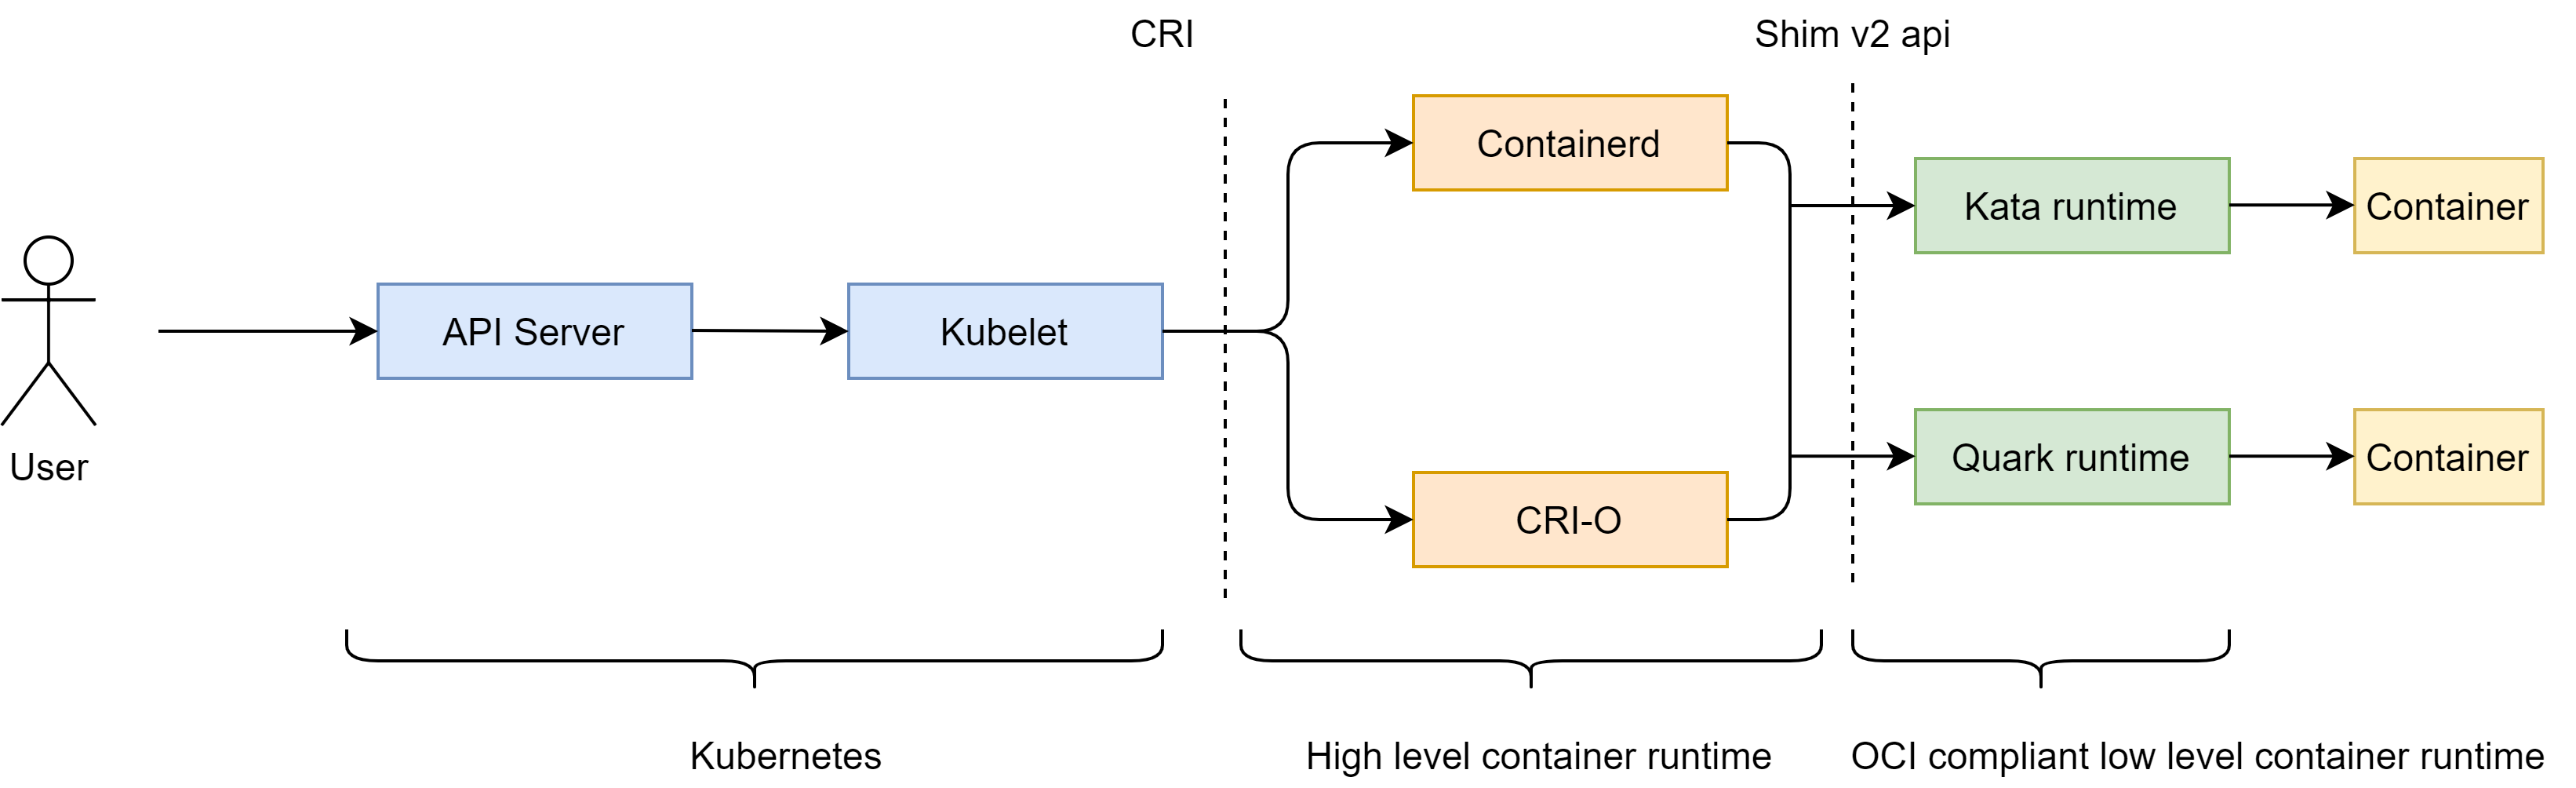
\includegraphics[width=0.8\textwidth]{images/k8s.PNG}
  \caption[Kubernetes architecture and runtime communication interface]{Kubernetes architecture and runtime communication interface}
  \label{fig:k8s}
\end{figure}

Standardized communication interfaces have been defined among the components in Figure~\ref{fig:k8s} for compatibility and scalability. The Kubelet utilizes the CRI interface~\cite*{cri-interface} to access services offered by the high-level runtime. Within the CRI, two gRPC interfaces are defined: the ImageService 
interface, responsible for managing images, and the RuntimeService interface, which manages containers and pods. Any high-level runtime integrated into the K8S ecosystem should implement the CRI interface. In addition, high-level runtimes support low-level runtimes that implement the shim interface~\cite*{shim_v2, cri0_shim_v2}. 
In Containerd, this interface is known as the shim v2 API~\cite*{shim_v2}, encompassing multiple ttrpc endpoints. It aims to abstract the implementation details of the low-level runtime and facilitate communication between higher-level runtimes and various lower-level runtimes.


\section{OCI runtime specification}

To ensure container portability and compatibility across runtimes, the Open Container Initiative (OCI) has introduced the OCI runtime specification~\cite*{oci-runtime-spec}. This specification outlines the procedure for low-level container runtimes to create and execute containers based on an 
application bundle and the methods for managing the container lifecycle. The high-level container runtime generates the application bundle from an image. It contains the container's root file system and a configuration file. This package is transferred to the low-level runtime via the Shim v2 API~\cite*{shim_v2}. 
The low-level runtime utilizes the metadata provided in the configuration file to create and configure the container. This metadata includes the following information: a process specification, metadata defining the container root file system, and mount information. The process specification defines 
the necessary metadata for creating the application or EXEC process, including environment variables, command line parameters, and STDIO type, among others. Mount information indicates the files or filesystems that should be mounted to the container's root filesystem during runtime. This may include 
Kubernetes secrets, k8s configuration files, and volumes~\cite*{k8s}. Additionally, on Linux platforms, the configuration file includes settings for hooks,  process security, and resource limits like rlimits and  AppArmor. These hooks are executable and executed by low-level container runtime at 
different stages of the container lifecycle (Figure~\ref{fig:Container_Lifecycle_state}).
\begin{figure}[htp]
  \centering
  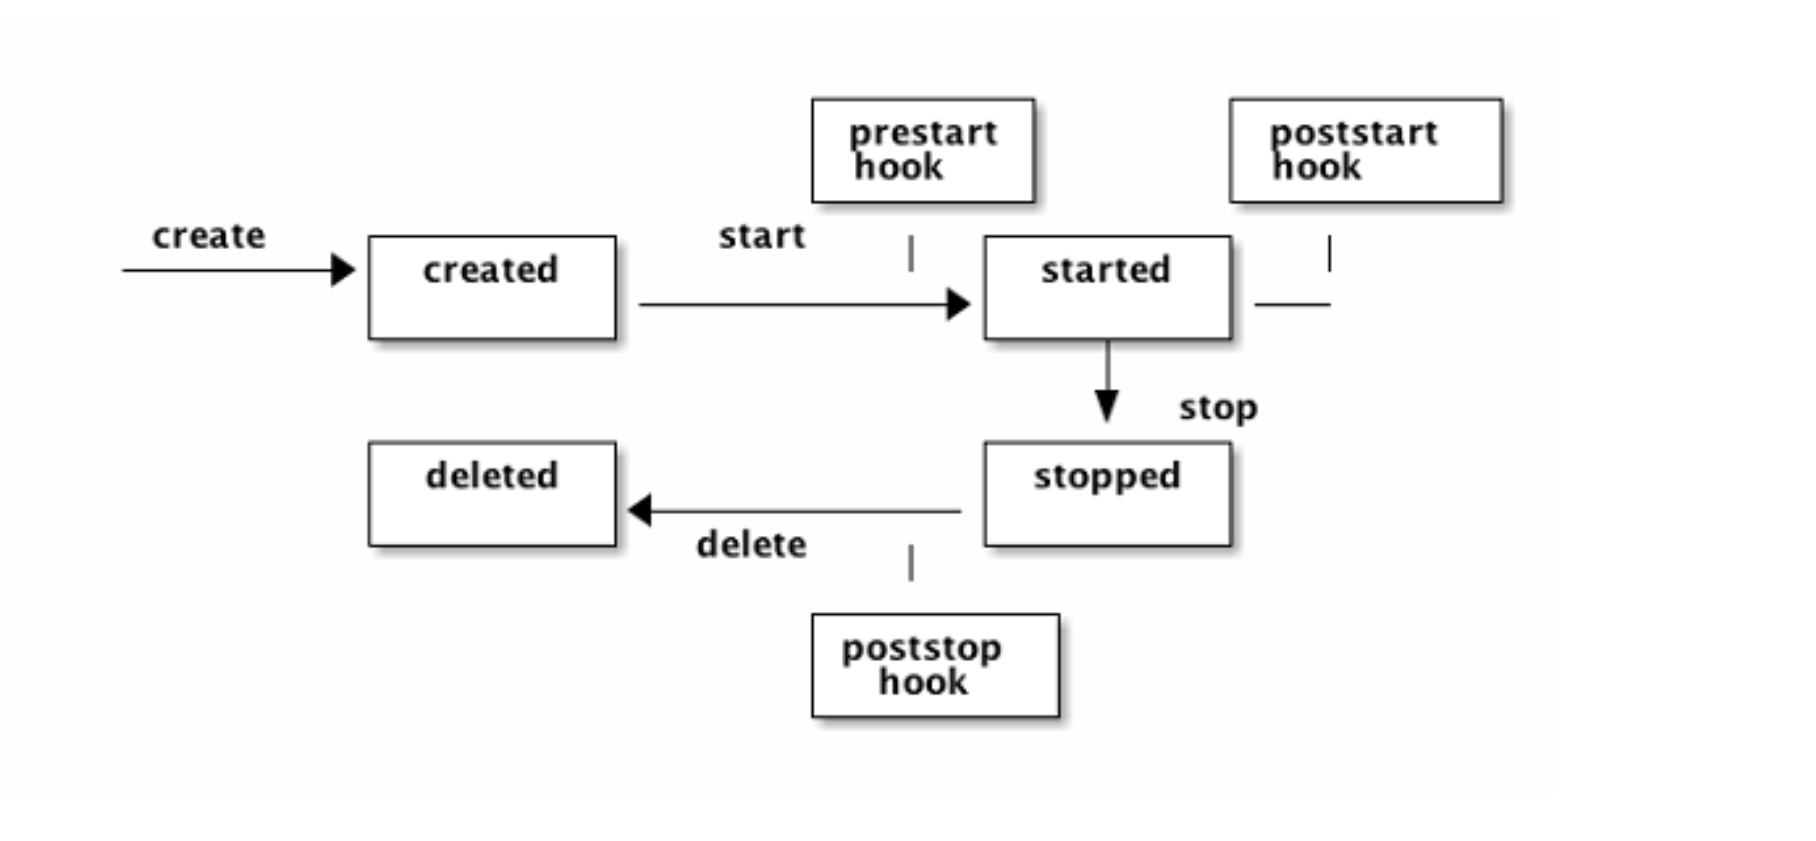
\includegraphics[width=0.8\textwidth]{images/Container_Lifecycle_state.PNG}
  \caption[Overview of container lifecycle]{Overview of container lifecycle}
  \label{fig:Container_Lifecycle_state}
\end{figure}

\section{Kata containers}
\label{sec:Kata}

Kata containers is an OCI-compliant low-level container runtime derived from combining two projects: Clear Containers and Hyper RunV~\cite*{Kata-Containers}. It offers an architecture for running containers in ultra-lightweight virtual machines. This architecture achieves performance similar to Runc and 
utilizes hardware virtualization technology to enhance the workload isolation~\cite*{9198653}.
\begin{figure}[htp]
  \centering
  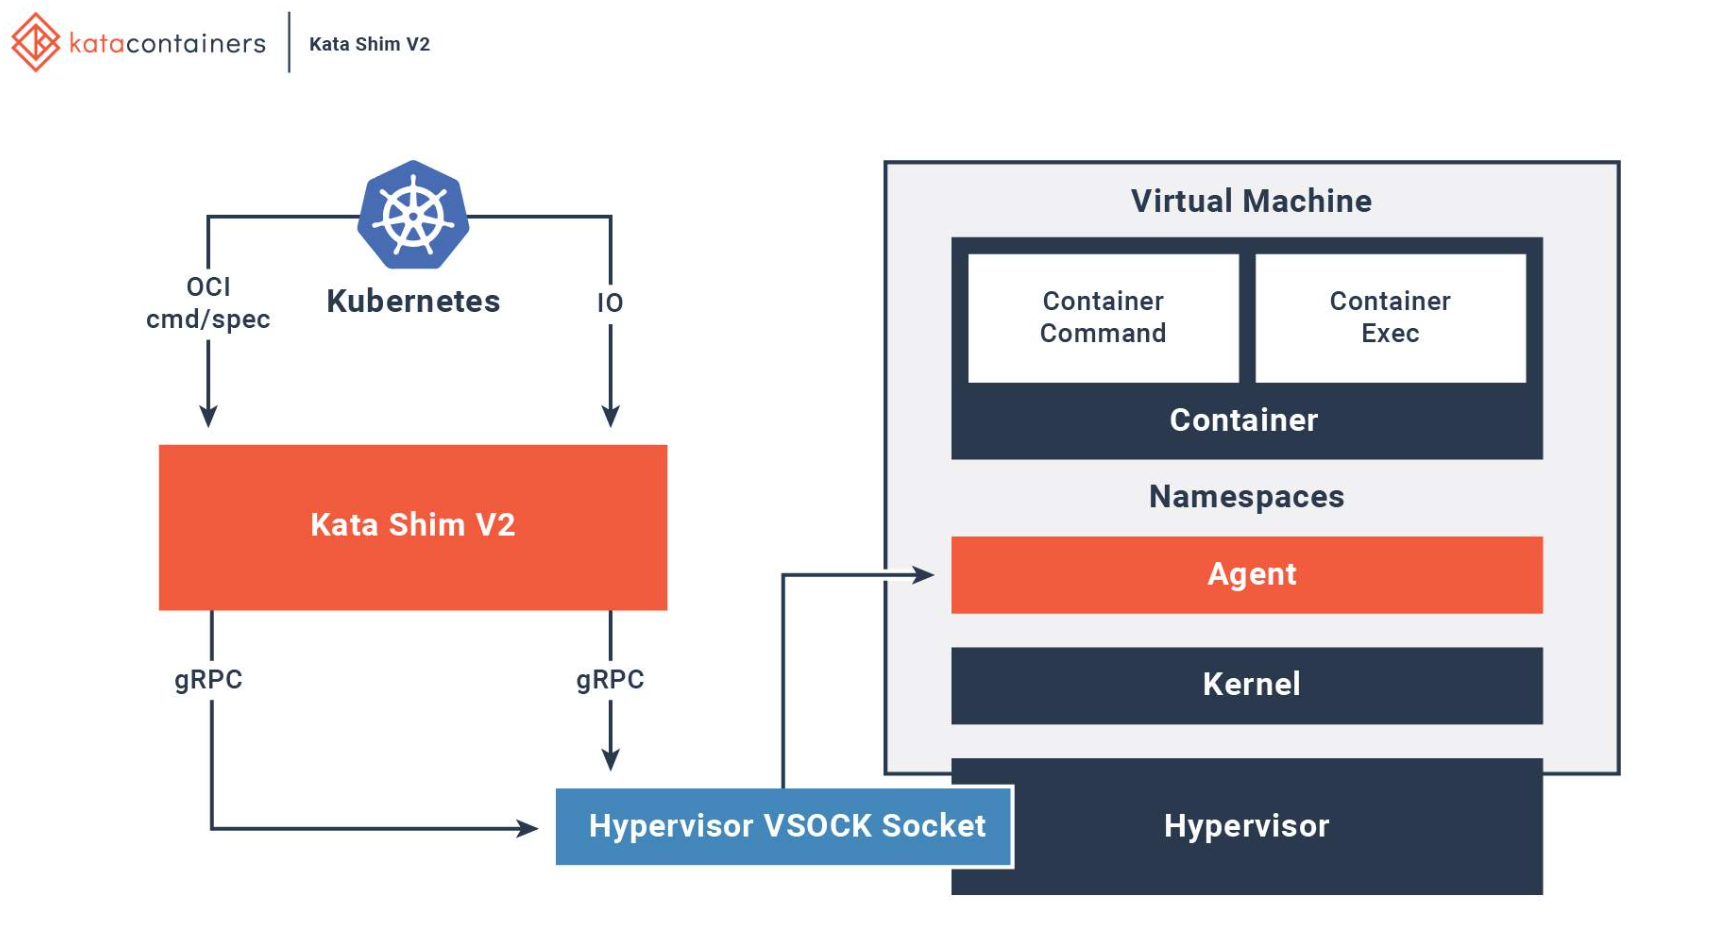
\includegraphics[width=0.6\textwidth]{images/kata.PNG}
  \caption[Kata containers architecture]{Kata containers architecture from~\cite*{Kata-Containers} }
  \label{fig:kata}
\end{figure}
Figure~\ref{fig:kata} presents the latest version (2.0) architecture of Kata Containers~\cite*{Kata_arch}. It consists of six elements: Kubernetes, high-level container runtime, Kata shim v2, hypervisor, guest kernel, and agent. In Section~\ref{sec:k8s}, both Kubernetes and the high-level container 
runtime are described. Kata shim v2 is a merging of multiple components in version 1.0, including the Kata shim, the Kata proxy, and the OCI-compliant Kata runtime~\cite*{Kata_arch}. It implements the shim v2 interface. Therefore, Containerd~\cite*{containerd} can issue commands to it. Within the 
virtual machine, Kata Container introduces a daemon named Kata agent, responsible for handling commands from Kata shim v2 and managing the running containers. Communication between Kata shim v2 and the Kata agent is facilitated through the VM's vsocket interface and the gRPC protocol. Furthermore, the 
Kata container utilizes a highly customized guest kernel that includes only the necessary services for running containers to achieve a low boot time and small memory footprint.


\section{Quark containers}
\label{sec:Quark}
Quark containers~\cite*{quark} is an OCI-compliant container runtime written in the Rust language. It shares a similar architecture with the Kata container, ensuring an equivalent level of container isolation. 
The difference is that the Qaurk uses an application kernel (also known as the forward kernel) as a guest OS. It implements some system calls and forwards others to the host. In comparison to the Kata containers that employ a dedicated kernel as the guest OS, 
the application kernel eliminates unnecessary code. Consequently, Quark has a smaller memory footprint and faster startup time~\cite*{quark_performance_report}. Moreover, Quark has developed the Ucall and Qcall interfaces to facilitate communication with the host. This approach efficiently avoids expensive VM exits when 
forwarding system calls to the host.

\begin{figure}[htp]
  \centering
  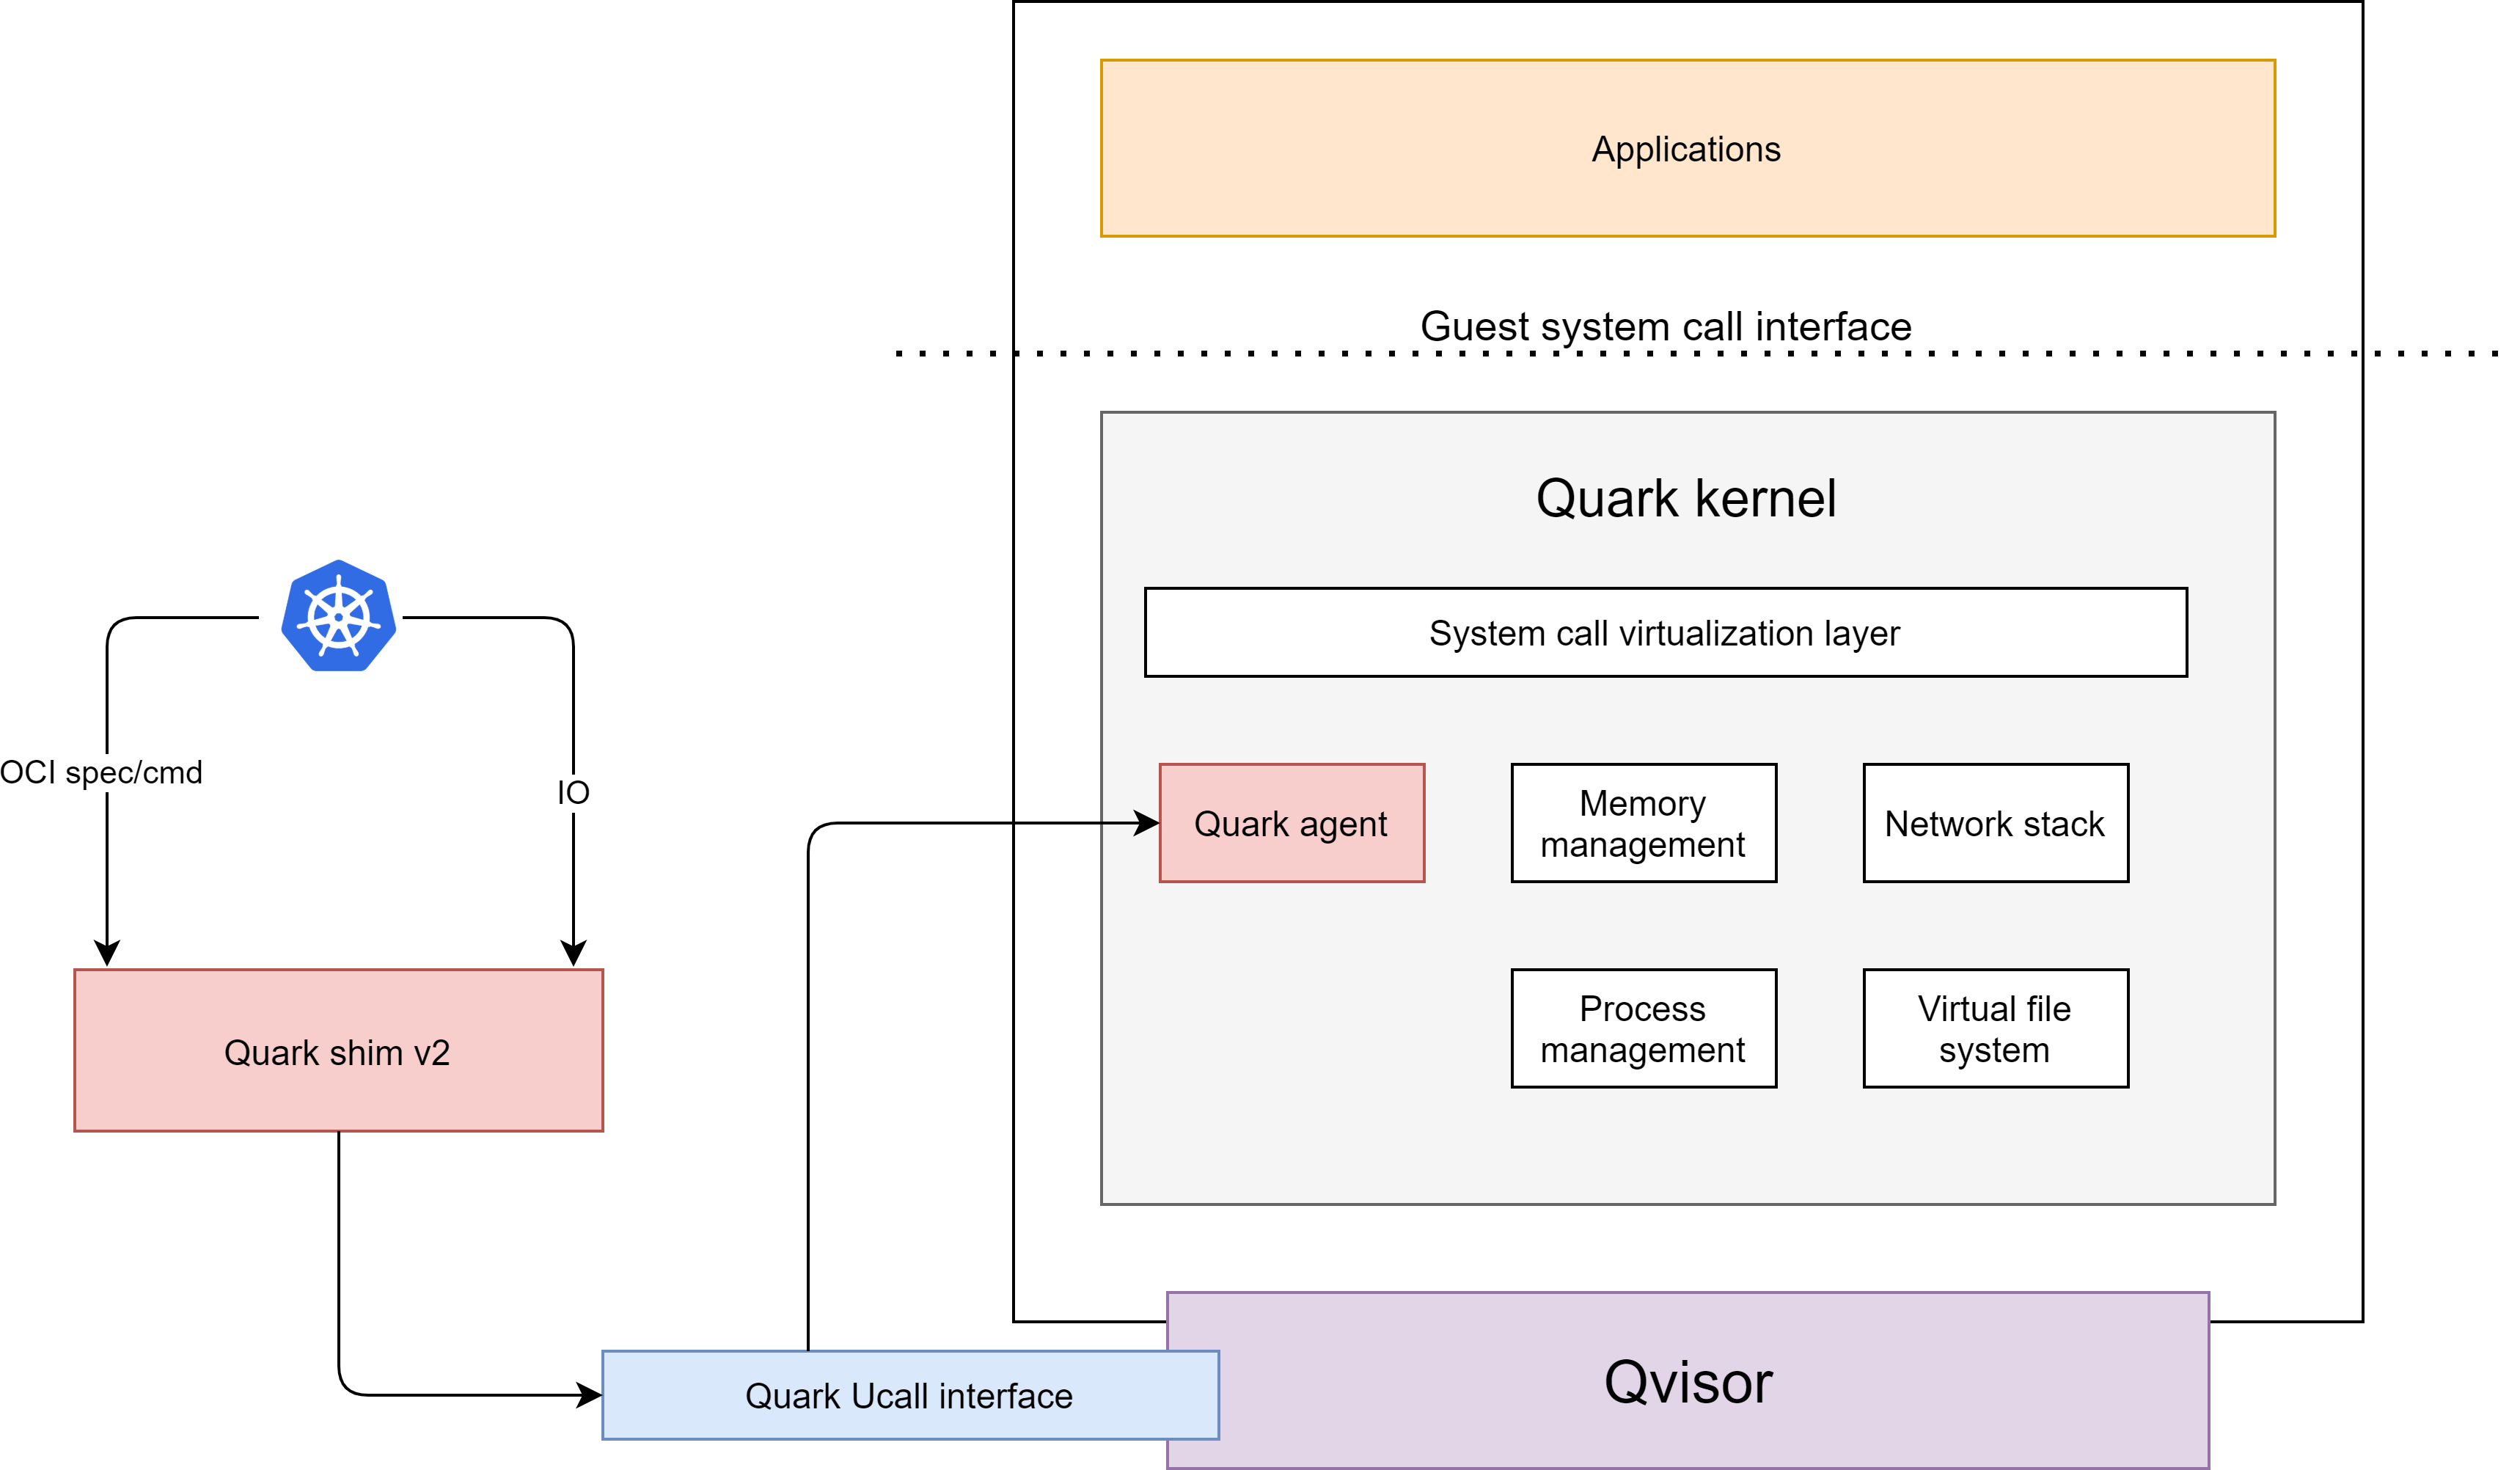
\includegraphics[width=0.6\textwidth]{images/QUARK_ARCH.PNG}
  \caption[Quark containers architecture]{Quark containers architecture}
  \label{fig:QUARK_ARCH}
\end{figure}


The architecture of the Quark container, as depicted in Figure~\ref{fig:QUARK_ARCH}, comprises five elements: Kubernetes~\cite*{k8s}, the high-level container runtime, Quark shim v2, Qvisor, and Qkernel. The description of Kubernetes and the high-level container runtime can be found in Section~\ref{sec:k8s}. 
Similarly to the Kata shim, the Quark shim is an OCI-compliant ttrpc server implemented in accordance with the Shim v2 API. As a result, it is capable of executing commands from Containerd~\cite*{containerd}. These commands may include invoking Qvisor to create lightweight virtual machines for 
containers with Qkernel as the guest OS. Qvisor is a virtualmachine manager similar to Qemu. It utilizes the KVM API to create and manage VMs that use Qkernel as the guest OS. Qkernel, on the other hand, is a minimized application kernel that contains only the necessary code. It implements process 
management, memory management, file system, and network stack. Notably, Qkernel utilizes the host operating system and Qvisor to manage physical devices, thereby avoid sophisticated IO handling and physical memory management. In addition, Qkernel implements most of the Linux system calls, which can be triggered by 
guest processes using the X86 syscall instruction. To accept the request from the Quark shim,  Qkernel implements a socket server called Quark agent. It uses Ucall 
and Qcall interfaces to communicate with Quark shim. Unlike the Kata agent, which operates as a user space process, the Quark agent is integrated within the Qkernel, and its code is part of the Qkernel binary.



\begin{figure}[htp]
  \centering
  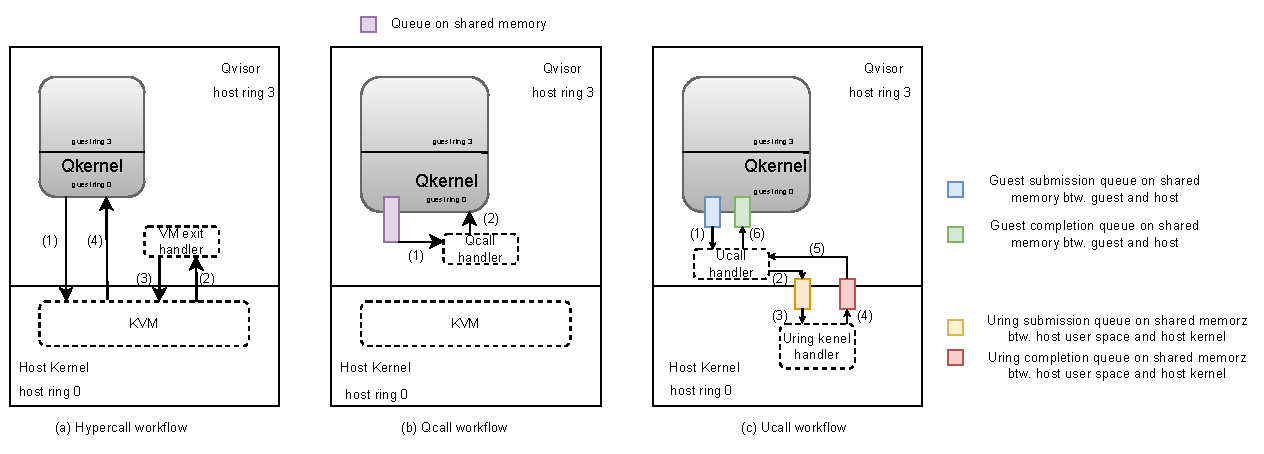
\includegraphics[width=1\textwidth]{images/hypercall_qcall_ucall.pdf}
  \caption[Workflow of Hypercall, Qcall, and Ucall]{Workflow of Hypercall, Qcall, and Ucall}
  \label{fig:hypercall_qcall_ucall}
\end{figure}


The workflow of Hypercall, Qcall, and Ucall is depicted in Figure~\ref{fig:hypercall_qcall_ucall}. Hypercall serves as the traditional mechanism for guests to communicate with the Virtual Machine Monitor (VMM). Qkenrel employs Hypercall to access services in Qvisor, like file opening and IO 
initialization. Figure~\ref{fig:hypercall_qcall_ucall}a illustrates the workflow of Hypercall. Upon triggering Hypercall, the CPU mode is changed from the guest ring 0  to the host ring 0. Subsequently, the KVM examines the Virtual Machine Control Block to determine the reason for the VM exit and 
forwards the Hypercall to the Qvisor running in host ring 3. Following the processing of the Hypercall, the Qvisor requests the KVM to resume guest execution.

Executing a Hypercall incurs significant overhead due to multiple world switches. To address this, Quark offers an asynchronous mechanism known as Qcall as an alternative approach for communicating with Qvisor. As depicted in Figure~\ref{fig:hypercall_qcall_ucall}(b), this mechanism consists of a 
shared memory queue between the Qkernel and the Qvisor and an IO thread in Qvisor. The shared queue facilitates the transfer of requests from Qkernel to Qvisor. The IO thread is responsible for retrieving the requests from the queue and notifying or awakening the Qkernel thread once the Qvisor completes the request. In summary,   
this mechanism allows Qkernel to access services in Qvisor asynchronously, eliminating the need for VM exit. 

The host operating system is responsible for performing IO read and write operations on physical devices. Therefore, Quark introduces the Ucall mechanism for communicating with the host kernel. This mechanism utilizes the Linux io\_uring and shared queues between Qvisor and Qkernel. It supports
both synchronous and asynchronous IO operations. Figure~\ref{fig:hypercall_qcall_ucall} explains the workflow of this mechanism. Initially, a Qkernel thread submits an IO request to the guest submission queue (Figure ~\ref{fig:hypercall_qcall_ucall}c (1)). Subsequently, the Qvisor Ucall handler copies the request to the Uring submission queue 
(Figure~\ref{fig:hypercall_qcall_ucall} (2)). Once the Uring kernel handler completes processing the IO request, it places the result into the uring completion queue (Figure~\ref{fig:hypercall_qcall_ucall}c (3), (4)). The result includes a user\_data, which is submitted with the initial IO 
request and contains information about the Qkernel thread. Using this information, the Qvisor Ucall handler can notify or wake the corresponding Qkernel thread. Note that the notification occurs after the IO processing result has been copied to the guest completion 
queue (Figure~\ref{fig:hypercall_qcall_ucall}c (5), (6)).

\section{Trusted Execution Environment}

The hardware-assisted Trusted Execution Environment (TEE) establishes tamper-proof computing environments, often referred to as enclaves, that ensure the confidentiality and integrity of data. It safeguards security-sensitive applications against co-located attackers through verifiable boot mechanisms, 
CPU and memory isolation, trusted IO, and secure storage~\cite*{Hardware-supported-TEE}. This security guarantee relays on hardware. Consequently, compromising software layers, including the operating system and hypervisor, does not diminish the TEE's capacity to protect sensitive 
computations and data~\cite*{7345265}.


Hardware-based TEE models can be categorized into two main types: virtual machine-based TEE and process-based TEE~\cite*{10.3389/fcomp.2022.930741}. Examples of virtual machine-based TEEs include Intel TDX~\cite*{Intel_tdx_whitepaper} and AMD SEV SNP~\cite*{SEV_SNP_white_book}, whereas Intel SGX~\cite*{INTEL_SGX} is the most famous process-based TEE. 
While Intel SGX has a smaller TCB, it requires modifications to an application to split it into trusted and untrusted parts. This can result in a degraded user experience. In contrast, VM-based TEEs enable the execution of programs without modification. However, this approach increases the 
trusted computing base (TCB), making it more susceptible to attacks~\cite*{Execution_Environment_landscape}.

The following two sections provide an overview of VM-based TEE. We chose AMD SNP and INTEL TDX as examples because they will likely be widely used. An explanation of process-based TEEs is beyond the scope of this thesis. For further details on this topic, please refer to~\cite*{cryptoeprint:2016/086, 10.1145/2487726.2488370}.


\subsection{AMD SEV SNP}

AMD SEV SNP~\cite*{SEV_SNP_white_book} is AMD's latest virtual machine-based TEE solution. It retains the features of its predecessors, AMD SEV~\cite*{sev} and AMD SEV-ES~\cite*{sev_es}, namely virtual machine memory encryption, register state protection, and further adds integrity protection for 
encrypted memory.


SNP utilizes encryption to protect the memory of a virtual machine. When a service running in an enclave (VM) accesses memory, the AES-128 encryption engine embedded in the memory controller transparently encrypts or decrypts the memory using a memory encryption key.  This key is unique for each 
enclave and securely stored in the AMD secure processor (AMD SP) to prevent unauthorized access. Consequently, untrusted entities can only read the ciphertext on the enclave memory. To enable memory page sharing between enclaves or between enclaves and the hypervisor, SEV SNP introduces a new 
control bit known as the "C-bit" in the page table. This enables enclaves to determine which pages should be encrypted.


SNP introduces the Reverse Map Table (RMP) to protect the integrity of enclave memory. The RMP ensures that each physical page is exclusively owned by a single entity. In this case, only the designated owner of a page is granted the permission to modify its contents. Any change in ownership 
will result in SNP erasing the contents of that page. To this end, untrusted entities can only read the encrypted enlave memory, without the ability to make any modifications to it.

\begin{figure}[htp]
  \centering
  \begin{subfigure}[b]{0.65\textwidth}
      \centering
      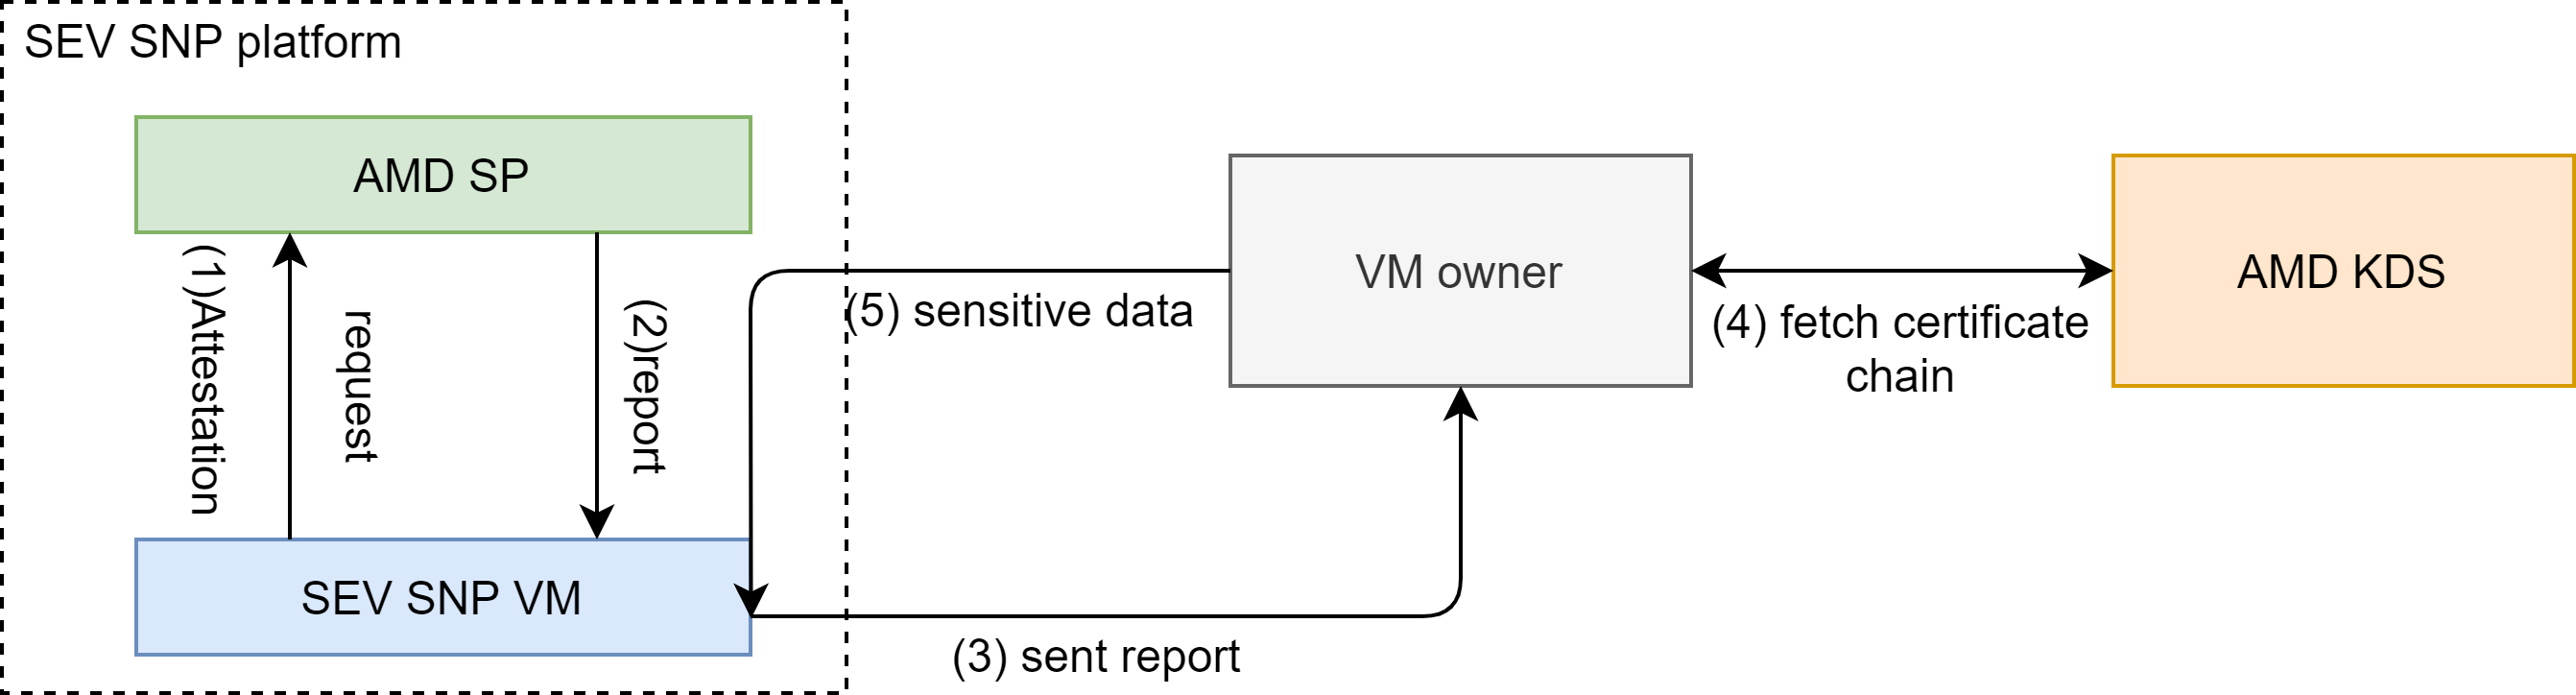
\includegraphics[width=\textwidth]{images/amd_attestation_workflow.PNG}
      \caption{Attestation workflow}
      \label{fig:amd_attestation_workflow}
  \end{subfigure}
  \hfill
  \begin{subfigure}[b]{0.3\textwidth}
      \centering
      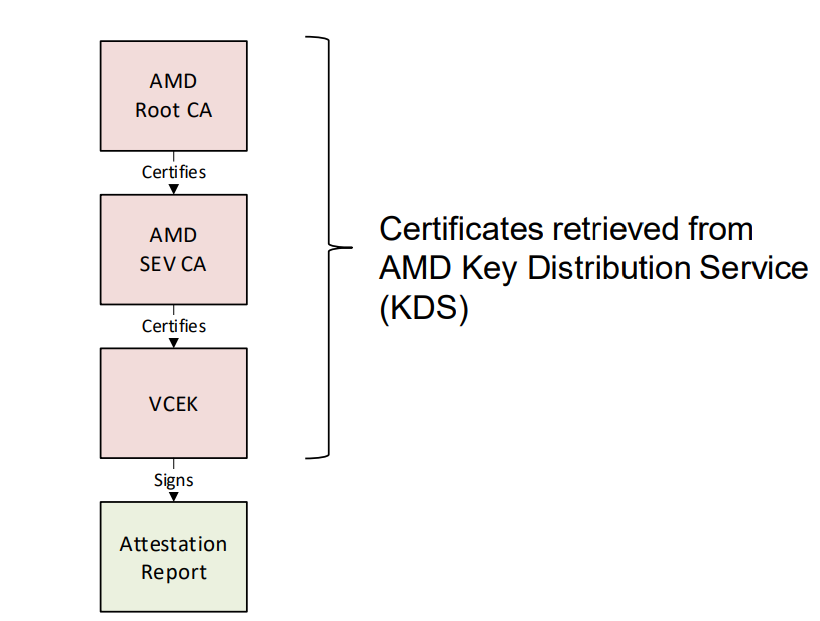
\includegraphics[width=\textwidth]{images/amd_snp_certificate_chain.PNG}
      \caption{Certificate chain (Figure from~\cite*{amd_Sev_snp_ppt})}
      \label{fig:amd_snp_certificate_chain}
  \end{subfigure}
  \hfill
     \caption[AMD SNP remote attestation]{AMD SNP remote attestation}
     \label{fig:amd_snp_atteation}
\end{figure}

SEV SNP also supports remote attestation, which allows the enclave owner to verify the authenticity of the VM. Unlike its predecessor, SNP enables enclaves to communicate with the AMD SP during runtime and request it to generate an attestation report. The communication between the enclave and AMD SP 
is facilitated by the SNP guest messages protocol~\cite*{snp_firmware, amd_sev_summarize}. The workflow for remote attestation is shown in Figure~\ref{fig:amd_attestation_workflow}. THE enclave first utilizes the SNP guest messages protocol to request a report from the AMD SP. The report is digitally signed using the Versioned Chip Endorsement Key (VCEK) and 
contains details such as the SP's measurement of the VM boot process, the SP firmware version, and a custom data. The VCEK is unique to each AMD platform because it is derived from platform-specific secrets and TCB versions. Once the enclave owner receives the report,  they can utilize the CHIP\_ID and TSB fields 
in the report to retrieve a certificate chain for the VCEK (Figure~\ref{fig:amd_snp_certificate_chain}) from the AMD Key Distribution Center. The certificate chain can be used to verify the signature of the report. Subsequently, by examining the remaining fields of the report, the enclave owner can determine whether the 
enclave is genuine.

\subsection{Intel TDX}
\label{subsec:tdx}

Intel TDX~\cite*{Intel_tdx_whitepaper} is a virtual machine-based TEE solution. Despite not being available on the market, some system-level software has already decided to adopt Intel TDX~\cite*{Kate_support_tdx, Linux_support_tdx}. Hence, we have provided a concise introduction to Intel TDX.
\begin{figure}[htp]
  \centering
  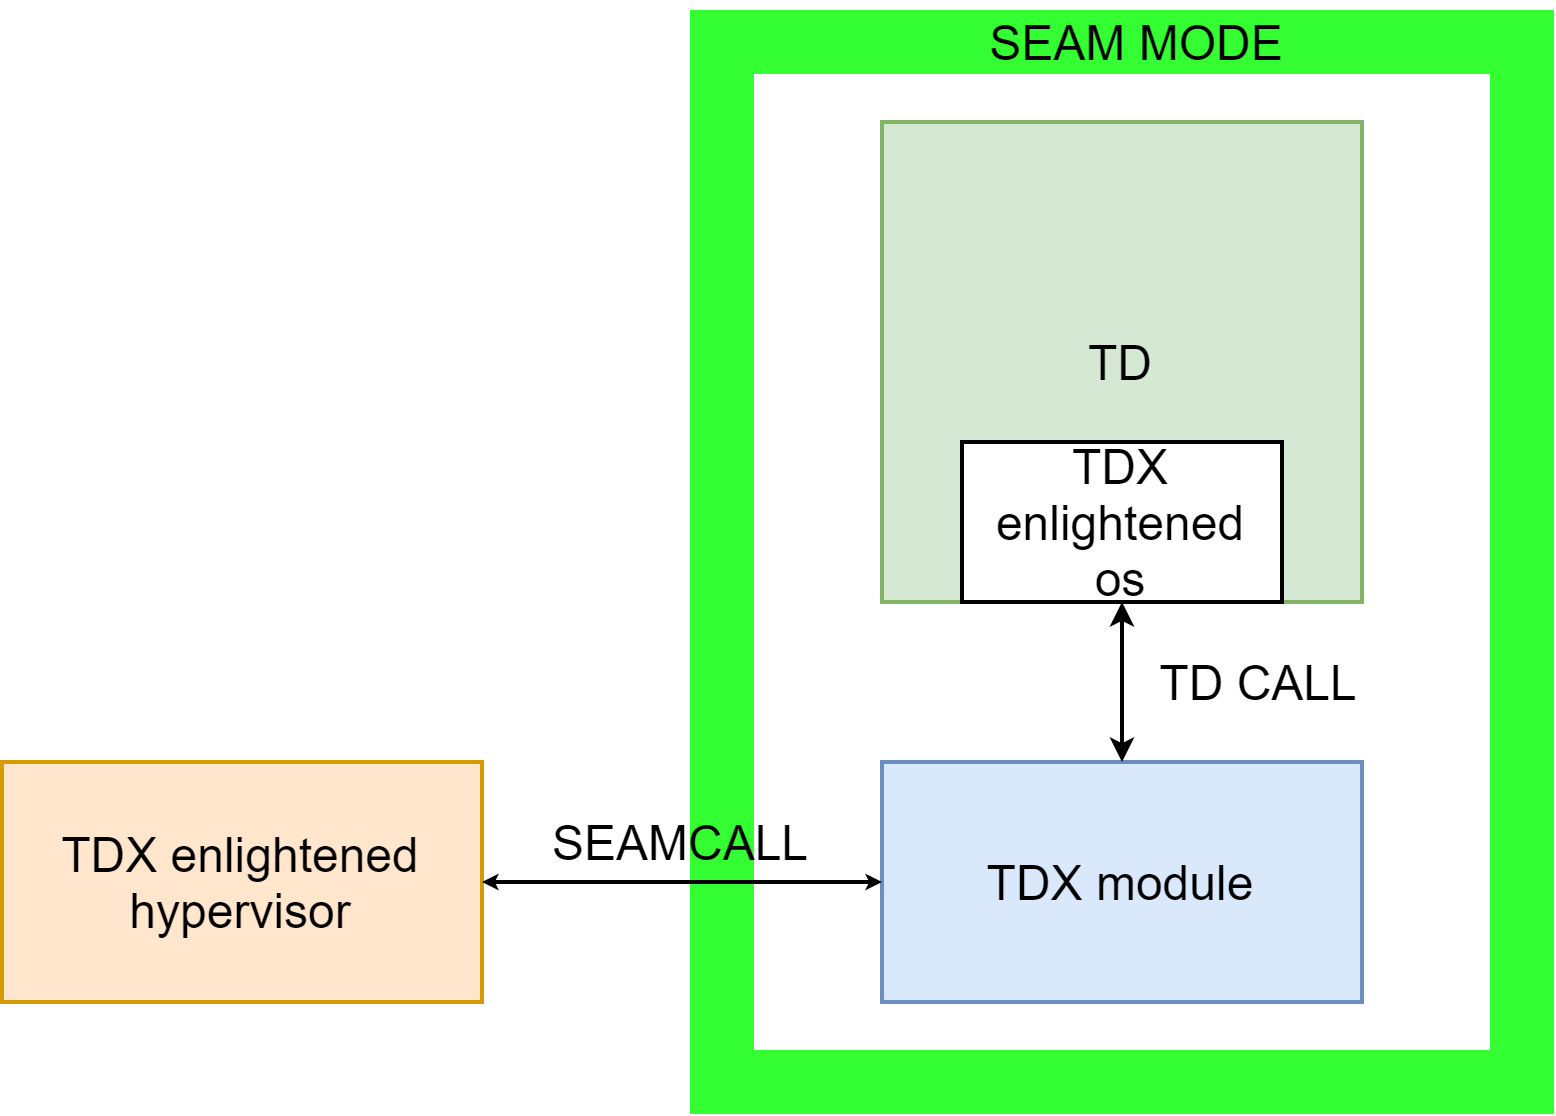
\includegraphics[width=0.4\textwidth]{images/td_arch.png}
  \caption[TDX architecture]{TDX architecture}
  \label{fig:td_arch}
\end{figure}
Intel TDX introduces a new CPU mode called Secure Arbitration Mode (SEAM). As shown in Figure~\ref{fig:td_arch}, the TDX module and all enclaves (TDs) run in this mode. It provides an isolated execution environment for TDs so that privileged software (VMM, OS) running in other modes cannot access 
the state and memory of the TDs. The TDX module manages the TDs and offers an interface for the VMM to send instructions to the TDs. The instructions include VMLAUNCH for initiating a TD and VMRESUME for restarting the TD. The TDX module can verify these instructions against the security 
policy to ensure the TDs are correctly operated.
\begin{figure}[htp]
  \centering
  \begin{subfigure}[b]{0.65\textwidth}
      \centering
      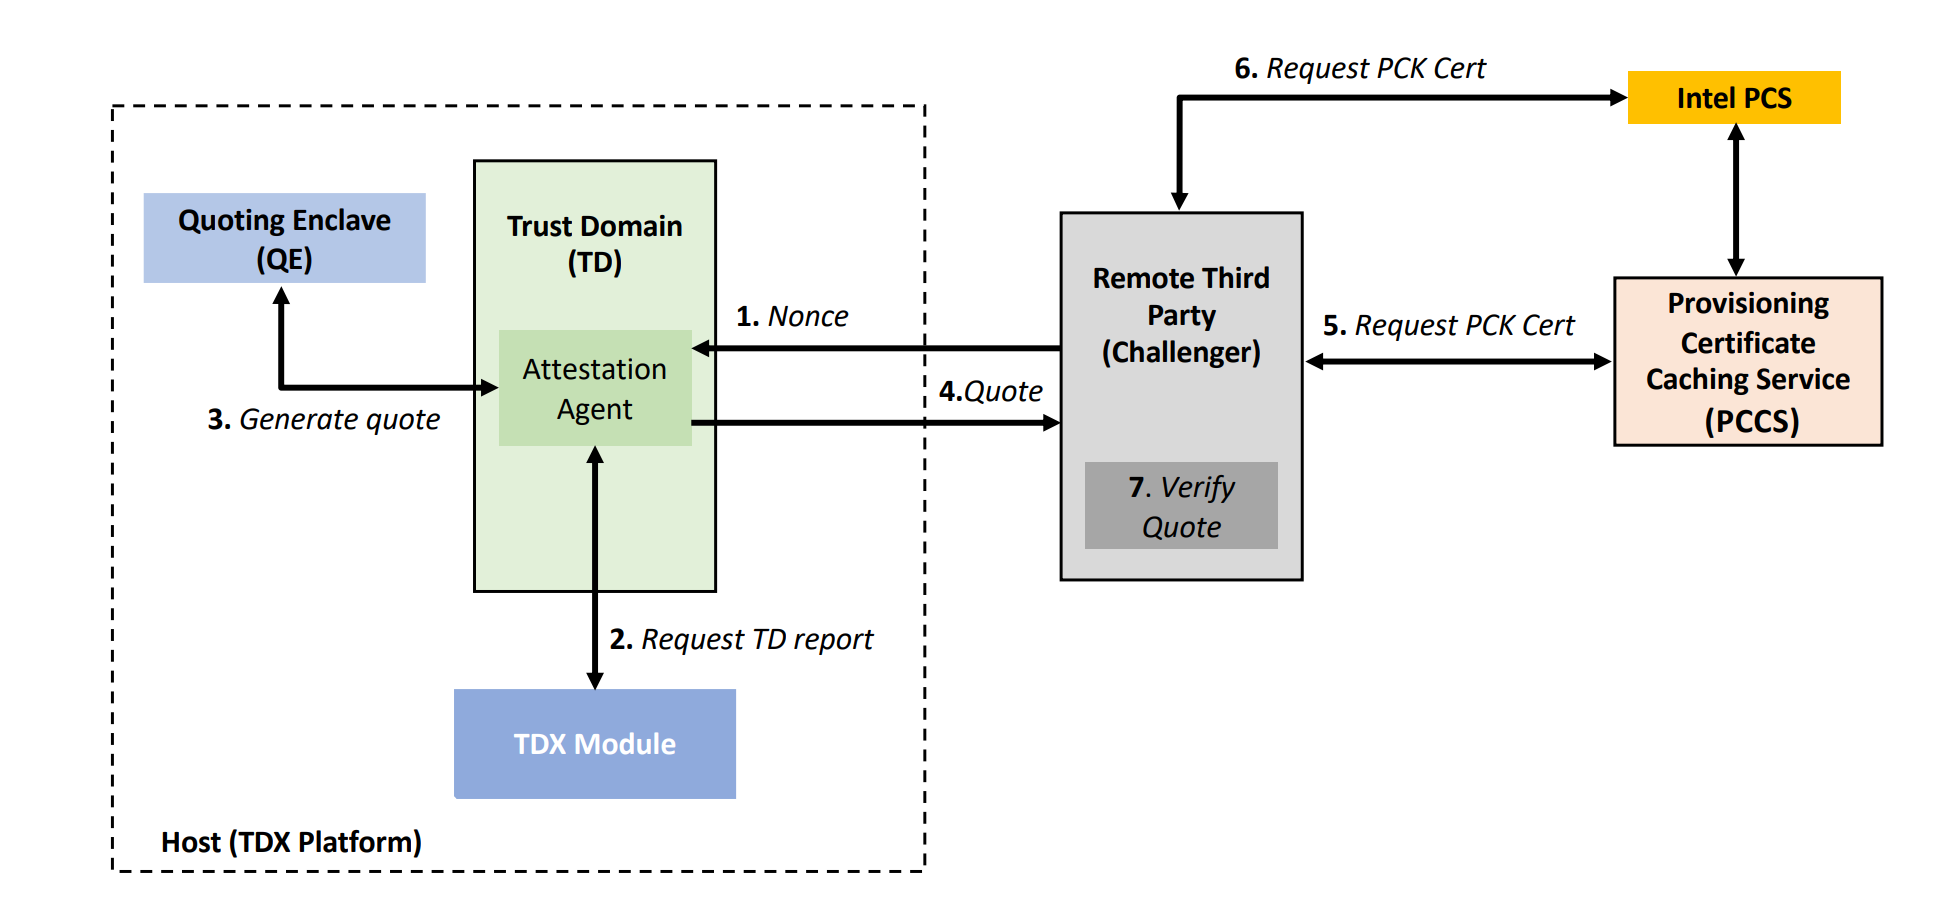
\includegraphics[width=\textwidth]{images/tdx_attestation_flow.png}
      \caption{Attestation workflow (from~\cite*{DBLP:journals/corr/abs-2303-15540})}
      \label{fig:tdx_attestation_flow}
  \end{subfigure}
  \hfill
  \begin{subfigure}[b]{0.3\textwidth}
      \centering
      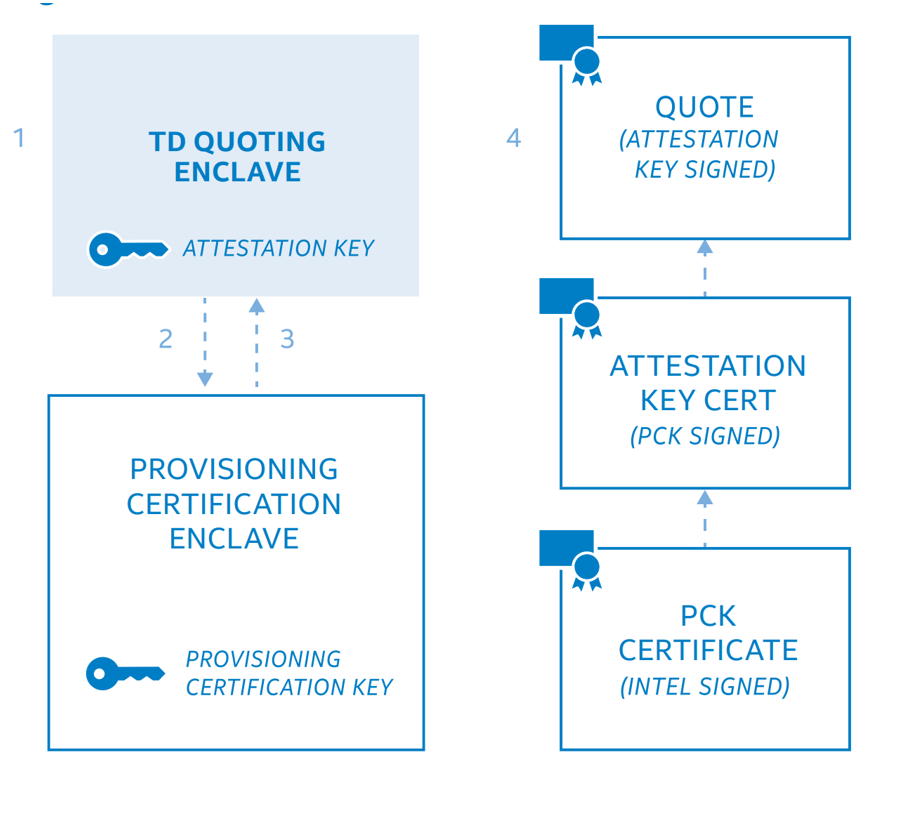
\includegraphics[width=\textwidth]{images/tdx_certi_chain.png}
      \caption{Certificate chain (from~\cite*{Intel_tdx_whitepaper})}
      \label{fig:tdx_certi_chain}
  \end{subfigure}
  \hfill
     \caption[Intel TDX remote attestation]{Intel TDX remote attestation}
     \label{fig:tdx_attestation}
\end{figure}
TDX also supports shared memory to facilitate communication between TDs or TD and untrusted entities like hypervisors. Like the SNP, each TD divides its memory into private and shared. External entities can access TD's shared memory in plaintext. This mechanism is implemented by introducing a 
new bit called the "shared bit" into the TD's page table entry and two EPTs, namely Secure EPT and Shared EPT. TD uses the shared bit to determine whether the Guest Physical Address (GPA) corresponds to shared memory. The secure EPT and shared EPT are responsible for converting private/shared 
GPAs to physical addresses. Note that only the private pages belonging to the secure EPT are encrypted by MKTME. Additionally, the Intel-TDX module hosts a data structure known as the Physical-Address-Metadata Table, which enforces page ownership. As a result, a page cannot be simultaneously 
mapped into the private memory of two TDs.


TDX leverages the Intel SGX attestation infrastructure for remote authentication~\cite*{Intel_tdx_whitepaper}, as shown in Figure~\ref{fig:tdx_attestation_flow}.
The workflow begins with the TD requesting the TDX Module to generate a local report using SEAMOPS [SEAMREPORT]. This report includes the TD's measurements, the SVN of the TDX-TCB element, custom data, etc. The integrity of this report is ensured by the CPU's HMAC key.
After generating the local report, the TD sends it to the quoting enclave,  which resides on the same platform. The quoting enclave first employs the EVERIFYREPORT command to request the CPU to verify the report's MAC. Then, it utilizes its attestation key to generate a signature based on the 
report data. The report data and the signature form a quote. Notably, the attestation key of the quoting enclave is certified by the Platform Certification Enclave (PCE) using the Provisioning Certification Key (PCK), which is itself certified by Intel.
Consequently, the signature of the quote forms a chain of signatures, as illustrated in Figure~\ref{fig:tdx_certi_chain}. The certificate chain can be used to verify the authenticity of this report off the platform. Subsequently, the TD transmits the quote to the TD owner. To verify the digital signature of the quote, 
the TD owner downloads the certificate chain from either the Platform Certificate Signing Service (PCCS) or Intel Provisioning Certification Service (PCS). Finally, by examining the report's contents, the TD owner can determine whether the TD is genuine.  For the detailed explanation of the Intel TDX remote attestation, we 
refer the reader to \cite*{Intel_tdx_whitepaper, 9448036, DBLP:journals/corr/abs-2303-15540}.

\subsection{Comparison of AMD SNP and Intel TDX}
Figure~\ref{fig:snp_tdx_compare} compares the features of Intel TDX and AMD SNP~\cite*{amd_sev_summarize}. In particular, we chose the most popular and widely used TEE, Intel SGX, 
as a reference.

\begin{figure}[htp]
  \centering
  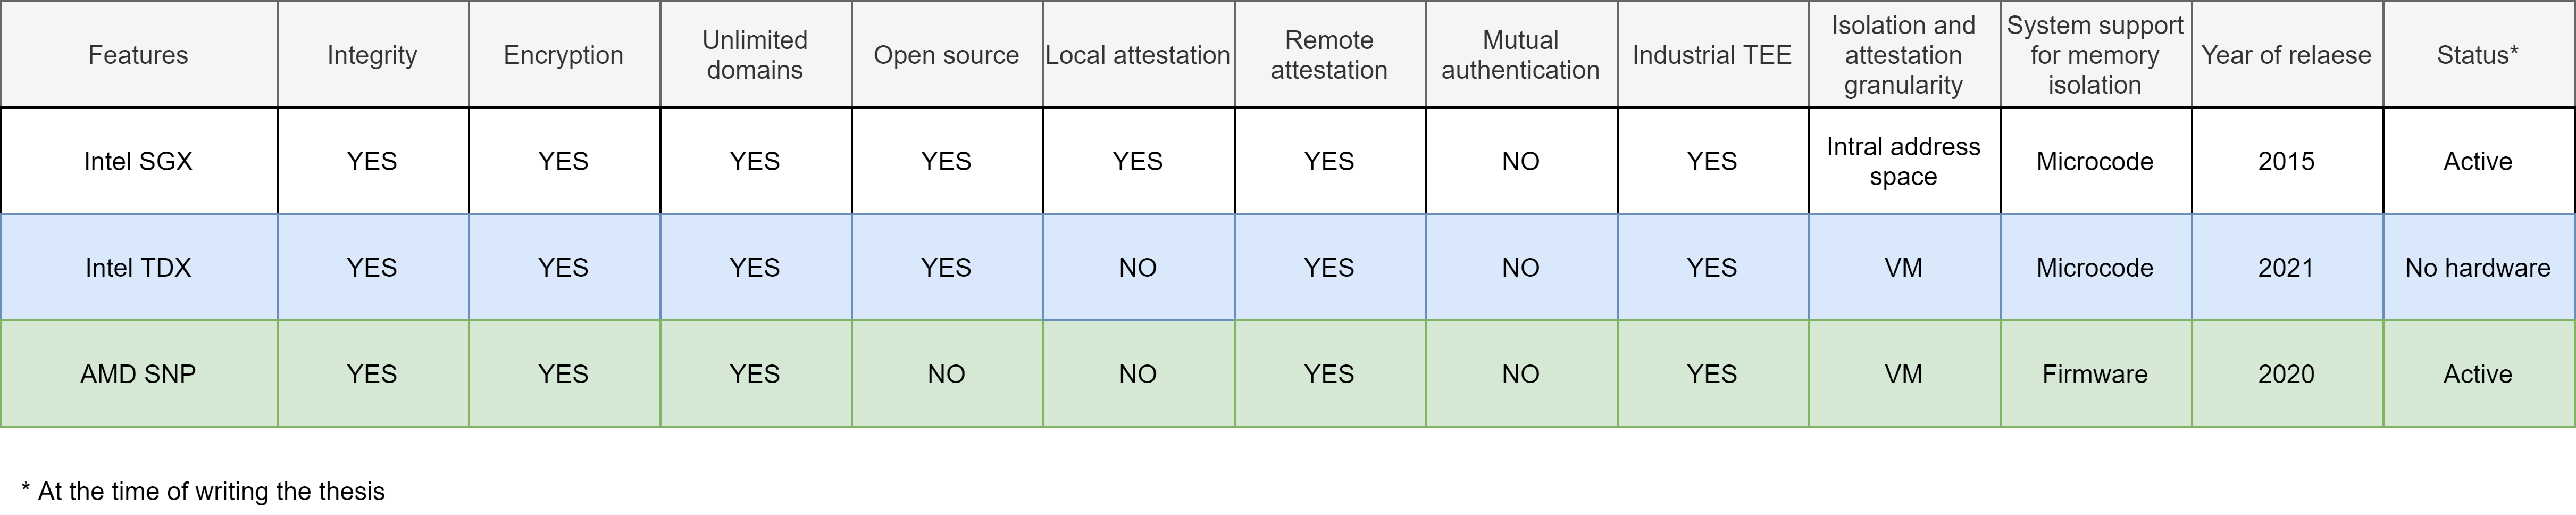
\includegraphics[width=1\textwidth]{images/snp_tdx_compare.png}
  \caption[Comparison of AMD SNP and Intel TDX]{Comparison of AMD SNP and Intel TDX}
  \label{fig:snp_tdx_compare}
\end{figure}




\section{KBS Attestation Protocol}
\label{sec:kbs}

KBS Attestation Protocol~\cite*{kbs_Attestation_protocol} is designed to establish trust between the Key Broker Client (KBC) and the Key Broker Service (KBS) and provide secrecy to the KBS.  The KBC is often referred to as an enclave, and the KBS serves as the secret manager. In this protocol, the KBC first utilizes the 
Request-Challenge-Attestation-Response (RCAR) method to authenticate to the KBS. Then, the HTTP GET request is employed to obtain the secrets from the KBS. Besides, the protocol employs TLS to prevent malicious attackers from hijacking the KBS address,  impersonating the KBS,  and injecting harmful 
data into the KBC. Specifically, the protocol requires that the KBS's public key be effectively distributed to the KBC so that the KBC can authenticate the KBS during the TLS handshake.

The protocol is divided into two phases. The first phase is the authentication phase, where the KBS authenticates the KBC using the KBC's attestation report. The second phase is the resource request phase, in which the KBS allows the KBC to retrieve a secret managed using the HTTP GET.  
The secret transmitted from the KBS to the KBC is encrypted using the KBC's public key. The public key is sent to the KBS with the KBC's attestation report during the first phase. Because the hash of the public key is included in the KBC's authentication report, the KBS can confirm that the public 
key is from the KBC and ensure that only the KBC can decrypt the encrypted secret. Additionally, the KBS assigns an HTTP cookie to the KBC during the authentication phase. This cookie associates the authentication result obtained in the first phase with the corresponding KBC. During the resource 
request phase, KBS uses this cookie to find the KBC's authentication result and considers it along with the policy to determine if a secret should be provided to the KBC. The following two diagrams detail how KBS and KBC work in phases 1 and 2:


\begin{figure}[htp]
    \centering
    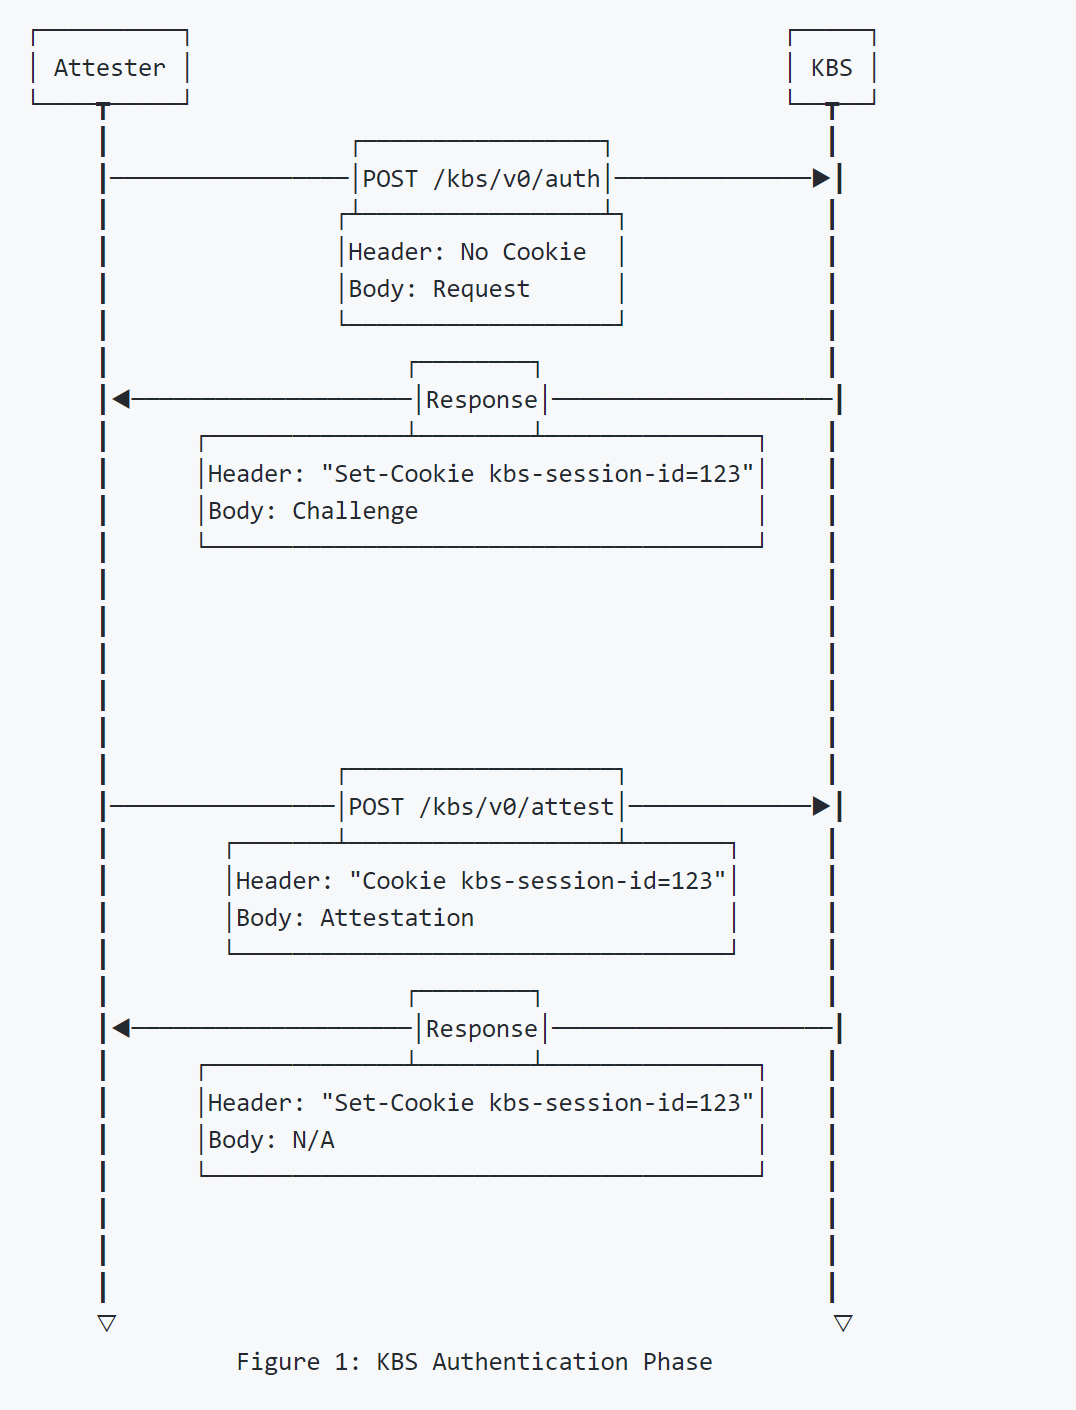
\includegraphics[width=0.5\textwidth]{images/attestation.PNG}
    \caption[Authentication phase]{Authentication phase}
    \label{fig:Authentication}
\end{figure}

As defined in Key Broke service attestation protocol, phase 1 (authentication phase) has 4 step: 
\begin{displayquote}
    \begin{enumerate}
        \item  Post /kbs/v0/auth: The KBC sends an HTTP Post whose body is a KBS Request JSON payload to KBS in order to initiate the attestation protocol. The payload contains The protocol version number supported by KBC, the type of HW-TEE platform where KBC is located.
        \item  Response: The KBS responds with the Challenge payload, which contains an attestation challenge (nonce) for the attester. KBC must place it in the evidence sent to the KBS in the next step to prevent replay attacks. Furthermore, the KBS also sends a session identifier to the KBC as an HTTP Cookie
        \item  Post /kbs/v0/auth: The KBC sends an HTTP Post request with a JSON payload called KBS Attestation and a Cookie set to the value received in the previous step. The payload contains the attestation evidence and the KBC’s public key.
        \item  Response: Upon successful attestation, the KBS replies to that request with an empty payload and sets the status code to 200. KBC can check the status code to determine if the authentication succeeds. 
    \end{enumerate}
\end{displayquote}

\begin{figure}[htp]
    \centering
    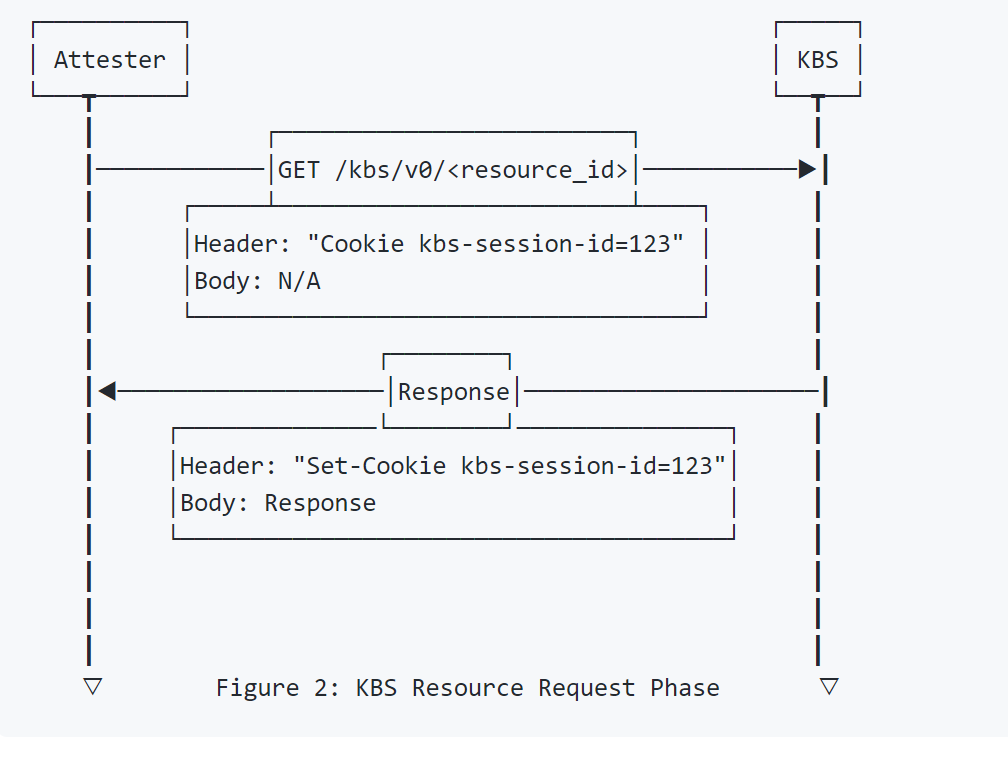
\includegraphics[width=0.5\textwidth]{images/resourcerequrie.PNG}
    \caption[Resource Requests phase]{Resource Requests phase}
    \label{fig:resourcerequrie}
\end{figure}
As defined in Key Broke service attestation protocol,  kbc can request resources or services from KBS during the second phase in the following way:
\begin{displayquote}
  To request a protected resource from the KBS, the attester sends a GET request to a resource-specific endpoint. If the attester can access the resource, the KBS will respond to the GET request with an HTTP response in which content is set to a KBS Response JSON payload.
\end{displayquote}


\section{Summary}
In this chapter, I first introduce k8s and the concept of high and low-level container runtimes. Next, I explain the standards and interfaces to enhance the scalability of k8s, namely CRI, OCI, and Shim V2 API. Additionally, I explain the architecture of the Kata and Quark container runtimes. 
Lastly, I illustrate TEE-related concepts like memory protection and remote attestation using AMD SNP and Intel TDX as examples.
\cleardoublepage

%%% Local Variables:
%%% TeX-master: "diplom"
%%% End:
